% ============================================================
% Module 04: LLM Fundamentals
% Custom Navasena Dark Beamer Theme
% Compiler: xelatex
% ============================================================
\documentclass[aspectratio=169,t]{beamer}

% ---- Fonts (xelatex) ----------------------------------------
\usepackage{fontspec}
\usepackage[sfdefault]{FiraSans}

% ---- Core packages ------------------------------------------
\usepackage{graphicx}
\usepackage{tikz}
\usetikzlibrary{positioning, shapes.geometric, arrows.meta, calc}
\usepackage{pgfplots}
\pgfplotsset{compat=1.18}
\usepackage{amsmath}
\usepackage{booktabs}
\usepackage{colortbl}
\usepackage{xcolor}
\usepackage{listings}

% ============================================================
% COLOR PALETTE (Navasena dark theme)
% ============================================================
\definecolor{nvbg}{HTML}{1A1A2E}        % dark navy background
\definecolor{nvdark}{HTML}{1A1A2E}     % alias for nvbg
\definecolor{nvcard}{HTML}{2D2D44}      % card / box background
\definecolor{nvgreen}{HTML}{76B900}     % primary accent
\definecolor{nvlightgreen}{HTML}{A3D944}% secondary accent
\definecolor{nvwhite}{HTML}{FFFFFF}
\definecolor{nvgray}{HTML}{AAAACC}      % muted text
\definecolor{nvdarkcard}{HTML}{23233A}  % slightly darker card
\definecolor{nvred}{HTML}{EF5350}       % accent red
\definecolor{nvorange}{HTML}{FF6F00}    % accent orange
\definecolor{nvblue}{HTML}{42A5F5}      % accent blue

% ============================================================
% LISTINGS STYLE
% ============================================================
\lstset{
  backgroundcolor=\color{nvcard},
  basicstyle=\ttfamily\small\color{nvwhite},
  keywordstyle=\color{nvgreen}\bfseries,
  stringstyle=\color{nvlightgreen},
  commentstyle=\color{nvgray}\itshape,
  numberstyle=\tiny\color{nvgray},
  numbers=left,
  numbersep=6pt,
  frame=none,
  breaklines=true,
  showstringspaces=false,
  tabsize=2,
  xleftmargin=8pt,
  xrightmargin=4pt,
}

% ============================================================
% BEAMER THEME — NAVASENA DARK
% ============================================================
\usetheme{default}
\usecolortheme{default}

% Background
\setbeamercolor{background canvas}{bg=nvbg}
\setbeamercolor{normal text}{fg=nvwhite}

% Frames
\setbeamercolor{frametitle}{fg=nvwhite, bg=nvbg}
\setbeamercolor{framesubtitle}{fg=nvgray, bg=nvbg}
\setbeamercolor{title}{fg=nvgreen}
\setbeamercolor{author}{fg=nvgray}
\setbeamercolor{date}{fg=nvgray}
\setbeamercolor{item}{fg=nvgreen}
\setbeamercolor{subitem}{fg=nvlightgreen}
\setbeamercolor{subsubitem}{fg=nvgray}
\setbeamercolor{block title}{fg=nvwhite, bg=nvcard}
\setbeamercolor{block body}{fg=nvwhite, bg=nvcard}

% Footline
\setbeamertemplate{footline}{%
  \hbox{%
    \begin{beamercolorbox}[wd=\paperwidth,ht=2.5ex,dp=1ex,leftskip=2em]{author in head/foot}%
      \color{nvgray}\small\textbf{LLM Fundamentals} \hfill \insertframenumber\,/\,\inserttotalframenumber
    \end{beamercolorbox}%
  }%
}

% Remove nav symbols
\setbeamertemplate{navigation symbols}{}

% ============================================================
% CUSTOM COMMANDS
% ============================================================
% \acttitle{Act N}{Title}{Subtitle/question}
\newcommand{\acttitle}[3]{%
  \begin{frame}[plain]
    \vspace{1.5cm}
    \begin{center}
      {\color{nvgreen}\Huge\bfseries Act #1}\\[1.2em]
      {\color{nvwhite}\Huge #2}\\[0.8em]
      {\color{nvgray}\Large #3}
    \end{center}
  \end{frame}%
}

% Section divider
\newcommand{\sectiontitle}[2]{%
  \begin{frame}[plain]
    \vspace{2cm}
    \begin{center}
      {\color{nvgreen}\Huge\bfseries #1}\\[1em]
      {\color{nvgray}\Large #2}
    \end{center}
  \end{frame}%
}

% Title page
\title{LLM Fundamentals}
\subtitle{Navasena Gen-ML Course}
\author{Navasena}
\date{}

% ============================================================
% DOCUMENT START
% ============================================================
\begin{document}

% Slide 1 — Title
\begin{frame}[plain]
  \vspace{1.2cm}
  \begin{center}
    {\color{nvgreen}\Huge\bfseries Module 04}\\[1.2em]
    {\color{nvwhite}\Huge\bfseries LLM Fundamentals}\\[0.6em]
    {\color{nvgray}\Large Large Language Models dengan Transformers}\\[2.2em]

    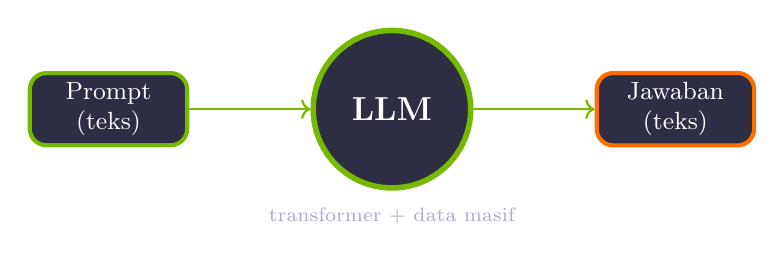
\begin{tikzpicture}[scale=0.9]
      \node[draw=nvgreen, fill=nvcard, rounded corners=6pt, line width=1.5pt,
            text=nvwhite, font=\small, minimum width=2cm, minimum height=0.9cm,
            align=center] (in) at (-4,0) {Prompt\\(teks)};
      \node[circle, fill=nvcard, draw=nvgreen, line width=2pt,
            minimum size=2cm, align=center] (llm) at (0,0)
            {\color{nvwhite}\large\bfseries LLM};
      \node[draw=nvorange, fill=nvcard, rounded corners=6pt, line width=1.5pt,
            text=nvwhite, font=\small, minimum width=2cm, minimum height=0.9cm,
            align=center] (out) at (4,0) {Jawaban\\(teks)};
      \draw[->,thick,color=nvgreen] (in) -- (llm);
      \draw[->,thick,color=nvgreen] (llm) -- (out);
      \node[color=nvgray, font=\scriptsize] at (0,-1.5) {transformer + data masif};
    \end{tikzpicture}

    \vspace{0.8em}
    {\color{nvgray}\small Achmad Zaenuri \quad $\cdot$ \quad \today}
  \end{center}
\end{frame}

% ── Act 1: Apa itu LLM? ───────────────────────────────────
\acttitle{1}{Apa itu LLM?}{Dari NLP ke model bahasa raksasa}

% Slide 2 — Definisi LLM
\begin{frame}{Definisi LLM}
  \framesubtitle{NLP itu bidang luas, LLM satu jenis model di dalamnya}
  \begin{columns}[T]
    \begin{column}{0.55\textwidth}
      \begin{itemize}
        \footnotesize
        \item \textbf{LLM} = \emph{Large Language Model}, jenis model \textbf{NLP} khusus
        \item Dilatih pada teks masif (miliaran kata dari internet)
        \item Berbasis arsitektur \textbf{transformer} + deep learning
        \item[\textcolor{nvgreen}{\checkmark}] \textbf{NLP}: bidang luas
        \item[\textcolor{nvgreen}{\checkmark}] \textbf{LLM}: satu jenis model di dalamnya
        \item Jago menulis, menerjemahkan, menjawab seperti manusia
      \end{itemize}
    \end{column}
    \begin{column}{0.42\textwidth}
      \begin{center}
      \resizebox{\linewidth}{!}{%
      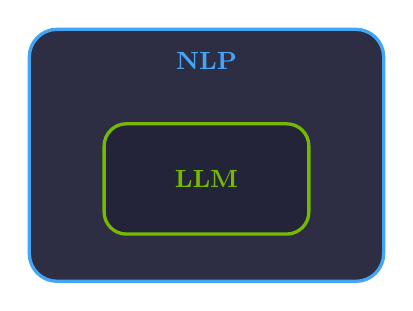
\begin{tikzpicture}
        \node[draw=nvblue, fill=nvcard, rounded corners=10pt, line width=1.2pt,
              text=nvblue, font=\small\bfseries, minimum width=4.5cm,
              minimum height=3.2cm] (nlp) at (0,0) {};
        \node[text=nvblue, font=\small\bfseries] at (0,1.2) {NLP};
        \node[draw=nvgreen, fill=nvdarkcard, rounded corners=8pt, line width=1.2pt,
              text=nvgreen, font=\small\bfseries, minimum width=2.6cm,
              minimum height=1.4cm, align=center] (llm) at (0,-0.3) {LLM};
      \end{tikzpicture}%
      }
      \end{center}
    \end{column}
  \end{columns}
  \vspace{0.4em}
  \begin{beamercolorbox}[rounded=true,shadow=false,sep=4pt]{block body}
    \small\color{white}
    Data masif $+$ \textbf{transformer} $=$ pemahaman bahasa luar biasa --- lompatan besar di dalam NLP.
  \end{beamercolorbox}
\end{frame}

% Slide 3 — Skala & Evolusi
\begin{frame}{Skala \& Evolusi}
  \framesubtitle{Skala parameter membantu, tapi data \& arsitektur juga menentukan}
  \begin{columns}[T]
    \begin{column}{0.5\textwidth}
      \begin{itemize}
        \footnotesize
        \item Evolusi: \textbf{n-gram} $\to$ \textbf{RNN/LSTM} $\to$ \textbf{Transformer} (2017)
        \item \textbf{Transformer} memproses kata secara paralel lewat \textbf{attention}, bukan satu per satu seperti RNN
        \item Umumnya makin banyak \textbf{parameter}, makin mampu menangkap pola (sampai titik tertentu)
        \item Kualitas \textbf{data}, arsitektur \& fine-tuning sama pentingnya
      \end{itemize}
    \end{column}
    \begin{column}{0.48\textwidth}
      \begin{center}
        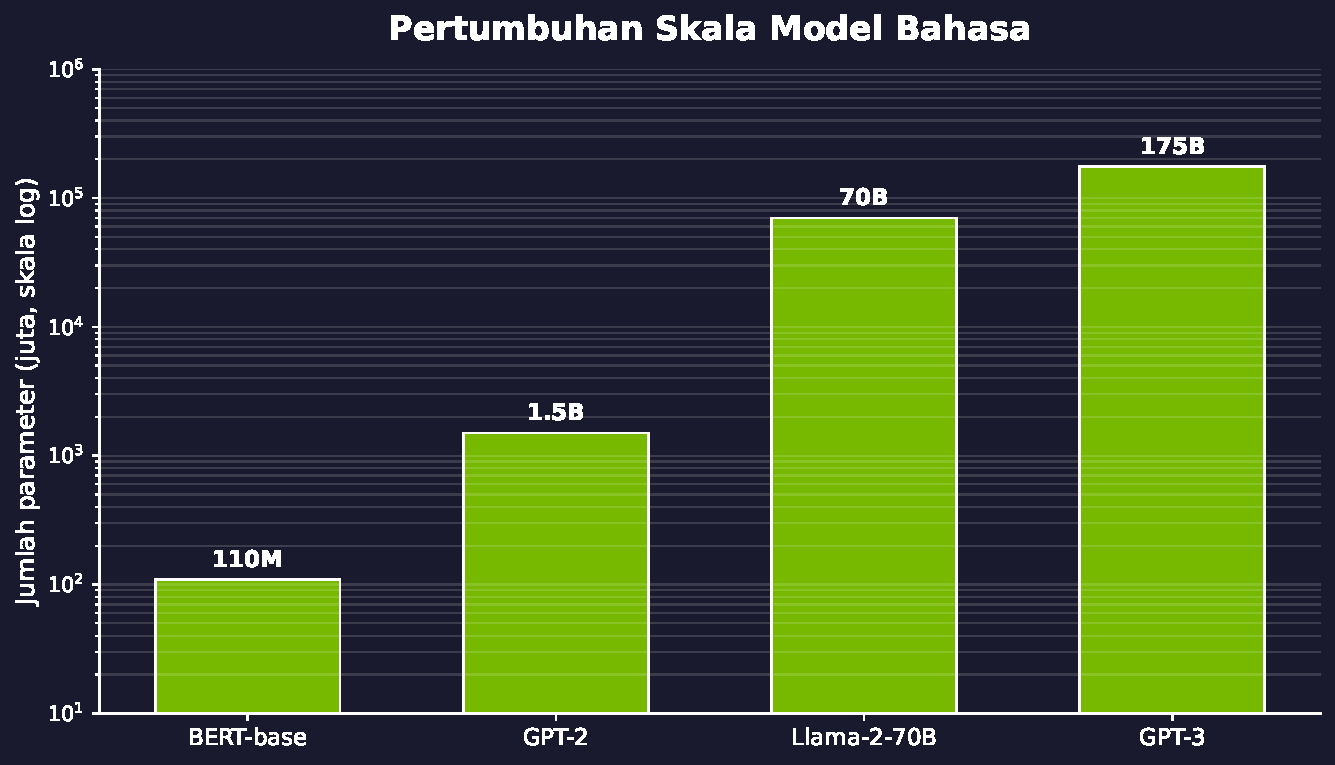
\includegraphics[width=\linewidth]{figures/model_scale.pdf}
      \end{center}
    \end{column}
  \end{columns}
  \vspace{0.3em}
  \begin{center}
    \textcolor{nvlightgreen}{\small Terobosan \textbf{Transformer} 2017 memicu ledakan ukuran: BERT 110M $\to$ GPT-3 175B}
  \end{center}
\end{frame}

% Slide 4 — Aplikasi LLM
\begin{frame}{Aplikasi LLM di Dunia Nyata}
  \framesubtitle{Satu model, banyak tugas bahasa}
  \begin{itemize}
    \item[\textcolor{nvgreen}{\checkmark}] \textbf{Chatbot} \& asisten: ChatGPT, Gemini, customer service
    \item[\textcolor{nvgreen}{\checkmark}] \textbf{Code generation}: bantu menulis \& menjelaskan kode
    \item[\textcolor{nvgreen}{\checkmark}] \textbf{Translation}: terjemahan antar bahasa
    \item[\textcolor{nvgreen}{\checkmark}] \textbf{Summarization}: meringkas dokumen panjang
    \item[\textcolor{nvgreen}{\checkmark}] \textbf{Question answering}: menjawab pertanyaan informatif
  \end{itemize}
  \vspace{0.6em}
  \begin{beamercolorbox}[rounded=true,shadow=false,sep=6pt]{block body}
    \centering\small\color{nvlightgreen}
    Satu \textbf{LLM} bisa mengerjakan banyak tugas bahasa sekaligus tanpa dilatih ulang per tugas.
  \end{beamercolorbox}
\end{frame}

% ── Act 2: Cara Kerja LLM ─────────────────────────────────
\acttitle{2}{Cara Kerja LLM}{Apa yang terjadi di balik layar}

% Slide 5 — Tokenization
\begin{frame}{Tokenization: Teks Menjadi Angka}
  \framesubtitle{Langkah pertama: memecah teks jadi token}
  \begin{columns}[T]
    \begin{column}{0.5\textwidth}
      \begin{itemize}
        \footnotesize
        \item Model tidak baca huruf; ia baca \textbf{token}
        \item \textbf{Token} sering berupa subword (potongan kata)
        \item Tiap \textbf{token} dipetakan ke sebuah \textbf{ID} angka
        \item Kata umum $=$ 1 token; kata jarang dipecah jadi beberapa
      \end{itemize}
    \end{column}
    \begin{column}{0.48\textwidth}
      \centering
      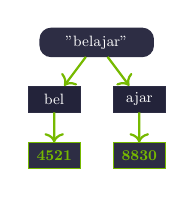
\begin{tikzpicture}[scale=0.6, every node/.style={transform shape}]
        \node[draw=nvcard, fill=nvcard, rounded corners=4pt, text=white,
              font=\small, minimum width=2.4cm, minimum height=0.6cm] (raw) at (0,1.4) {"belajar"};
        \node[draw=nvcard, fill=nvdarkcard, text=nvwhite, font=\small,
              minimum width=1.1cm, minimum height=0.55cm] (t1) at (-0.9,0.2) {bel};
        \node[draw=nvcard, fill=nvdarkcard, text=nvwhite, font=\small,
              minimum width=1.1cm, minimum height=0.55cm] (t2) at (0.9,0.2) {ajar};
        \node[draw=nvgreen, fill=nvcard, text=nvgreen, font=\small\bfseries,
              minimum width=1.1cm, minimum height=0.55cm] (id1) at (-0.9,-1.0) {4521};
        \node[draw=nvgreen, fill=nvcard, text=nvgreen, font=\small\bfseries,
              minimum width=1.1cm, minimum height=0.55cm] (id2) at (0.9,-1.0) {8830};
        \draw[->,thick,color=nvgreen] (raw) -- (t1);
        \draw[->,thick,color=nvgreen] (raw) -- (t2);
        \draw[->,thick,color=nvgreen] (t1) -- (id1);
        \draw[->,thick,color=nvgreen] (t2) -- (id2);
      \end{tikzpicture}
      \\[0.2em]
      {\tiny\color{nvgray}(ID hanya ilustrasi)}
    \end{column}
  \end{columns}
  \vspace{0.2em}
  \begin{center}
    \textcolor{nvlightgreen}{\small Komputer tidak mengerti kata; semua diubah jadi \textbf{token ID} dulu.}
  \end{center}
\end{frame}

% Slide 6 — Embedding & Transformer
\begin{frame}{Embedding \& Transformer}
  \framesubtitle{Dari ID angka ke prediksi kata berikutnya}
  \begin{center}
    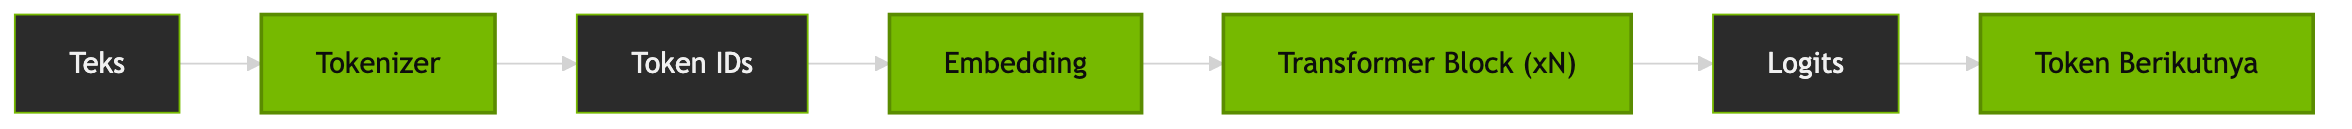
\includegraphics[width=0.82\textwidth]{figures/llm_architecture.png}
  \end{center}
  \vspace{0.4em}
  \begin{itemize}
    \footnotesize
    \item Tiap \textbf{token ID} $\to$ \textbf{embedding} (vektor angka); kata mirip makna $\to$ vektor mirip
    \item Vektor diproses berlapis lewat \textbf{transformer block}; output $=$ prediksi \textbf{token} berikutnya
  \end{itemize}
\end{frame}

% Slide 7 — Attention
\begin{frame}{Attention secara Intuitif}
  \framesubtitle{Model belajar kata mana yang saling merujuk}
  \begin{columns}[T]
    \begin{column}{0.48\textwidth}
      \begin{itemize}
        \footnotesize
        \item \textbf{Attention} $=$ model "memperhatikan" kata paling relevan
        \item Saat memproses 1 kata, ia menimbang semua kata lain
        \item Model belajar \textbf{"itu"} merujuk ke \textbf{"buku"}, bukan "meja"
        \item Kunci agar LLM paham konteks kalimat panjang
      \end{itemize}
    \end{column}
    \begin{column}{0.5\textwidth}
      \begin{center}
      \resizebox{\linewidth}{!}{%
      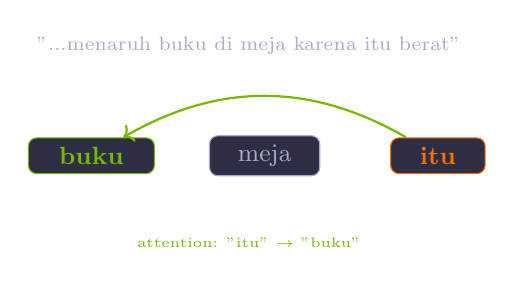
\begin{tikzpicture}
        \node[text=nvgray, font=\scriptsize] at (0,2) {"...menaruh buku di meja karena itu berat"};
        \node[draw=nvgreen, fill=nvcard, rounded corners=3pt, text=nvgreen,
              font=\small\bfseries, minimum width=1.6cm] (buku) at (-2,0.6) {buku};
        \node[draw=nvgray, fill=nvcard, rounded corners=3pt, text=nvgray,
              font=\small, minimum width=1.4cm] (meja) at (0.2,0.6) {meja};
        \node[draw=nvorange, fill=nvcard, rounded corners=3pt, text=nvorange,
              font=\small\bfseries, minimum width=1.2cm] (itu) at (2.4,0.6) {itu};
        \draw[->,thick,color=nvgreen, bend right=30] (itu) to[bend right=30] (buku);
        \node[text=nvgreen, font=\tiny] at (0,-0.5) {attention: "itu" $\to$ "buku"};
      \end{tikzpicture}%
      }
      \end{center}
    \end{column}
  \end{columns}
  \vspace{0.3em}
  \begin{beamercolorbox}[rounded=true,shadow=false,sep=4pt]{block body}
    \centering\small\color{white}
    Attention membuat model fokus pada kata yang benar-benar relevan, bukan semua sama rata.
  \end{beamercolorbox}
\end{frame}

% Slide 8 — Generasi & Sampling
\begin{frame}{Generasi Teks \& Sampling}
  \framesubtitle{Menulis satu token demi satu token}
  \begin{center}
    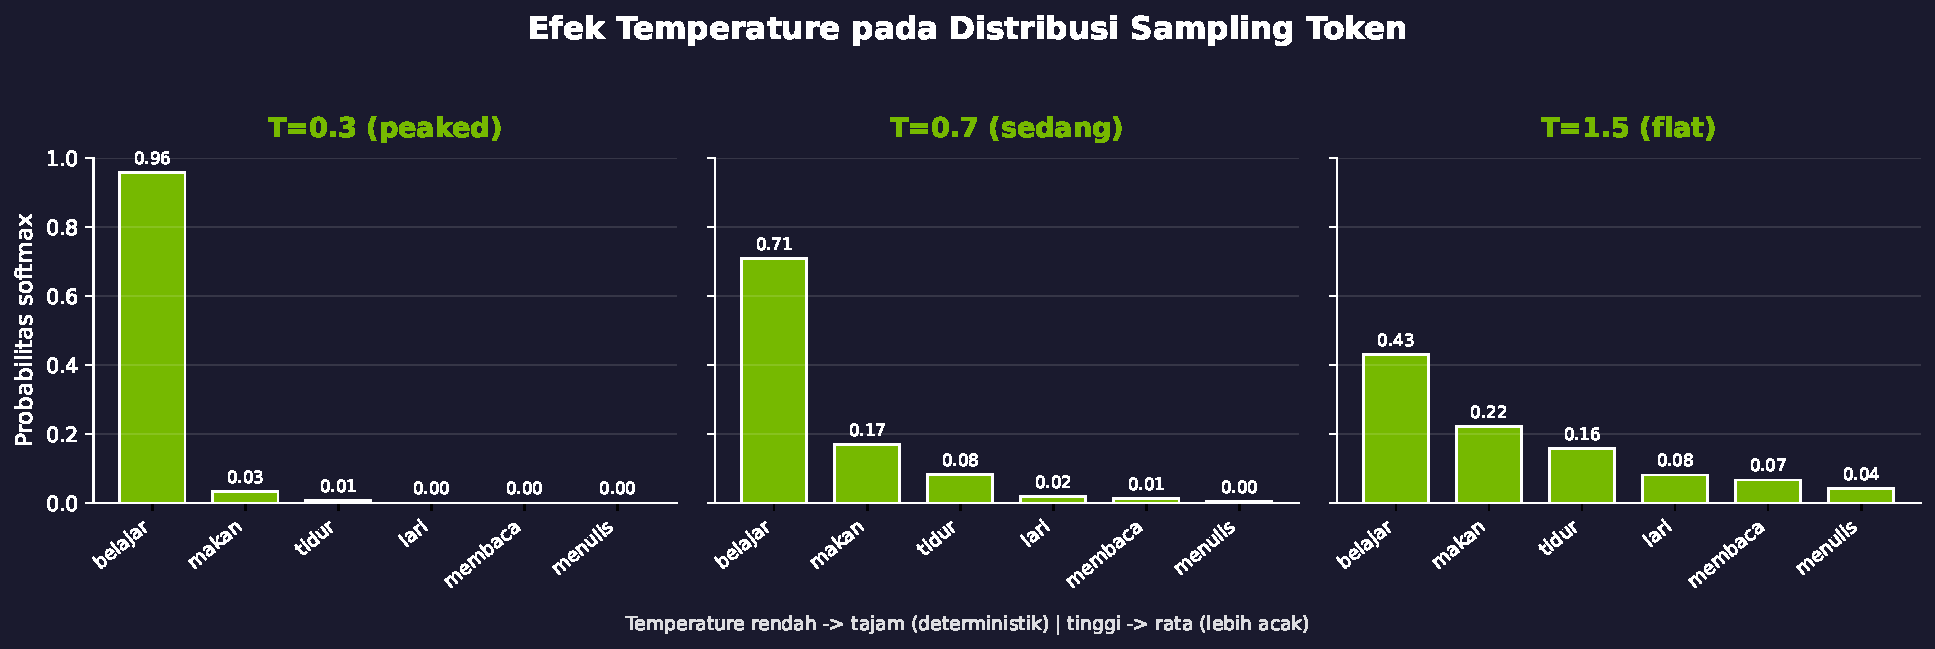
\includegraphics[width=0.92\textwidth]{figures/sampling.pdf}
  \end{center}
  \vspace{0.1em}
  \begin{columns}[T]
    \begin{column}{0.5\textwidth}
      \begin{itemize}
        \footnotesize
        \item LLM \textbf{autoregressive}: prediksi 1 \textbf{token} lalu ulang
        \item Tiap token baru jadi input token selanjutnya
      \end{itemize}
    \end{column}
    \begin{column}{0.48\textwidth}
      \begin{itemize}
        \footnotesize
        \item \textbf{temperature}: rendah $=$ fokus, tinggi $=$ kreatif/acak
        \item \texttt{do\_sample=True} $\to$ pilih token acak-terbobot
      \end{itemize}
    \end{column}
  \end{columns}
\end{frame}

% ── Act 3: Memakai LLM dengan HuggingFace ─────────────────
\acttitle{3}{Memakai LLM dengan HuggingFace}{Dari teori ke kode}

% Slide 9 — Ekosistem HuggingFace
\begin{frame}{Ekosistem HuggingFace}
  \framesubtitle{Pustaka open-source untuk LLM}
  \begin{itemize}
    \item[\textcolor{nvgreen}{\checkmark}] Library \textbf{transformers}: API standar memuat \& menjalankan model
    \item[\textcolor{nvgreen}{\checkmark}] \textbf{Model Hub}: ribuan model siap pakai, gratis di-\emph{download}
    \item[\textcolor{nvgreen}{\checkmark}] Tiap model punya \textbf{model card}: deskripsi, lisensi, cara pakai
    \item[\textcolor{nvgreen}{\checkmark}] Model datang lengkap dengan \textbf{tokenizer} \& \textbf{config}
  \end{itemize}
  \vspace{0.6em}
  \begin{beamercolorbox}[rounded=true,shadow=false,sep=6pt]{block body}
    \centering\small\color{nvlightgreen}
    Tidak perlu melatih dari nol --- ambil model siap pakai dari Hub.
  \end{beamercolorbox}
\end{frame}

% Slide 10 — pipeline vs Load Manual
\begin{frame}[fragile]{pipeline vs Load Manual}
  \framesubtitle{Dua cara memanggil model}
  \begin{columns}[T]
    \begin{column}{0.44\textwidth}
      \begin{itemize}
        \footnotesize
        \item \textbf{pipeline}: cepat, cukup sebut task + nama model
        \item \textbf{AutoModel + AutoTokenizer}: manual, lebih fleksibel
        \item pipeline cocok untuk eksperimen cepat
        \item Load manual: kontrol penuh atas tokenizer \& \textbf{inference}
      \end{itemize}
    \end{column}
    \begin{column}{0.54\textwidth}
      \begin{lstlisting}[language=Python, basicstyle=\ttfamily\scriptsize\color{nvwhite}]
from transformers import pipeline

pipe = pipeline("text-generation",
                model="facebook/opt-350m")
pipe("My name is")
      \end{lstlisting}
    \end{column}
  \end{columns}
  \vspace{0.2em}
  \begin{center}
    \textcolor{nvlightgreen}{\small pipeline $=$ mudah \quad$\cdot$\quad AutoModel $=$ fleksibel \& terkontrol}
  \end{center}
\end{frame}

% Slide 11 — Model Gated & Login HF
\begin{frame}[fragile]{Model Gated \& Login HF}
  \framesubtitle{Akses model yang dibatasi}
  \begin{columns}[T]
    \begin{column}{0.54\textwidth}
      \begin{itemize}
        \footnotesize
        \item Sebagian model \textbf{gated}, contoh: \textbf{Llama-2} dari Meta
        \item Perlu setujui lisensi \& punya \textbf{token} akses HuggingFace
        \item Login dulu lewat \textbf{huggingface-cli login}
        \item Tujuan: lisensi, kontrol penggunaan, verifikasi pengguna
      \end{itemize}
    \end{column}
    \begin{column}{0.44\textwidth}
      \begin{lstlisting}[language=bash, basicstyle=\ttfamily\footnotesize\color{nvwhite}]
!huggingface-cli login
      \end{lstlisting}
      \vspace{0.4em}
      \begin{center}
        \textcolor{nvgreen}{\footnotesize token HF $\to$ akses model gated}
      \end{center}
    \end{column}
  \end{columns}
  \vspace{0.3em}
  \begin{beamercolorbox}[rounded=true,shadow=false,sep=4pt]{block body}
    \centering\small\color{white}
    Model gated butuh token: \textbf{login} dulu sebelum download.
  \end{beamercolorbox}
\end{frame}

% Slide 12 — Text Classification
\begin{frame}{Text Classification}
  \framesubtitle{Mekanik pipeline \& pentingnya fine-tuning}
  \begin{columns}[T]
    \begin{column}{0.5\textwidth}
      \begin{itemize}
        \footnotesize
        \item \texttt{pipeline("sentiment-analysis")} di atas \textbf{AutoModelForSequence\-Classification}
        \item \textbf{prajjwal1/bert-tiny} baru di-pretrain, \textbf{belum} punya head klasifikasi terlatih
        \item Akibatnya label $=$ \textbf{LABEL\_0/LABEL\_1}, score $\sim$0.5 (tebakan acak)
        \item Untuk sentimen nyata: pakai model \emph{fine-tuned} (mis. \texttt{distilbert} di \textbf{SST-2})
      \end{itemize}
    \end{column}
    \begin{column}{0.48\textwidth}
      \begin{center}
      \renewcommand{\arraystretch}{1.15}
      {\scriptsize
      \setlength{\tabcolsep}{3pt}
      \begin{tabular}{@{}p{0.58\linewidth}p{0.16\linewidth}p{0.14\linewidth}@{}}
        \toprule
        \rowcolor{nvcard!50}
        \textbf{Teks} & \textbf{Label} & \textbf{Score} \\
        \midrule
        I love working with language models! & LABEL\_1 & 0.535 \\
        This task is quite challenging. & LABEL\_1 & 0.510 \\
        The results are impressive and amazing. & LABEL\_1 & 0.522 \\
        \bottomrule
      \end{tabular}%
      }
      \end{center}
    \end{column}
  \end{columns}
  \vspace{0.3em}
  \begin{beamercolorbox}[rounded=true,shadow=false,sep=4pt]{block body}
    \centering\small\color{white}
    Head belum terlatih $\to$ output $\sim$0.5 (acak); butuh model \emph{fine-tuned} untuk sentimen nyata.
  \end{beamercolorbox}
\end{frame}

% ── Act 4: Aplikasi LLM ───────────────────────────────────
\acttitle{4}{Aplikasi LLM}{Membangun sesuatu yang berguna}

% Slide 13 — Chatbot dengan Gradio
\begin{frame}[fragile]{Chatbot dengan Gradio}
  \framesubtitle{Antarmuka chat dalam beberapa baris kode}
  \begin{columns}[T]
    \begin{column}{0.42\textwidth}
      \begin{itemize}
        \footnotesize
        \item \textbf{gr.ChatInterface} membuat tampilan chat siap pakai
        \item Fungsi menyusun \textbf{prompt} \texttt{"User: ...\textbackslash nAssistant:"}
        \item Parameter \textbf{history} disediakan Gradio (di sini diabaikan)
        \item \textbf{launch(share=True)} beri tautan publik
      \end{itemize}
    \end{column}
    \begin{column}{0.56\textwidth}
      \begin{lstlisting}[language=Python, basicstyle=\ttfamily\scriptsize\color{nvwhite}]
def chatbot_response(message, history):
    prompt = f"User: {message}\nAssistant:"
    return generate_text(prompt, model,
                         tokenizer, max_length=150)

iface = gr.ChatInterface(chatbot_response,
            title="Simple LLM Chatbot")
iface.launch(share=True)
      \end{lstlisting}
    \end{column}
  \end{columns}
\end{frame}

% Slide 14 — Few-shot Learning
\begin{frame}[fragile]{Few-shot Learning}
  \framesubtitle{Mengajari model lewat contoh di dalam prompt}
  \begin{columns}[T]
    \begin{column}{0.44\textwidth}
      \begin{itemize}
        \footnotesize
        \item Beri beberapa \textbf{contoh} langsung di dalam \textbf{prompt}
        \item Tanpa melatih ulang, model meniru pola
        \item Pola Q/A berulang, pertanyaan baru dibiarkan kosong
        \item Prompt lebih panjang $\to$ naikkan \textbf{max\_length}
      \end{itemize}
    \end{column}
    \begin{column}{0.54\textwidth}
      \begin{lstlisting}[language=Python, basicstyle=\ttfamily\scriptsize\color{nvwhite}]
Q: What is the capital of France?
A: The capital of France is Paris.

Q: What is the capital of Japan?
A: The capital of Japan is Tokyo.

Q: What is the capital of Italy?
A:    <- model melanjutkan
      \end{lstlisting}
    \end{column}
  \end{columns}
  \vspace{0.2em}
  \begin{center}
    \textcolor{nvlightgreen}{\small Contoh $>$ perintah: tunjukkan pola, model akan menirunya.}
  \end{center}
\end{frame}

% Slide 15 — Model Evaluation
\begin{frame}[fragile]{Model Evaluation}
  \framesubtitle{Mengukur kualitas output secara sederhana}
  \begin{columns}[T]
    \begin{column}{0.46\textwidth}
      \begin{itemize}
        \footnotesize
        \item Jalankan beberapa \textbf{test prompt} ke model
        \item Catat tiap \textbf{prompt}, \textbf{response}, \& panjang jawaban
        \item Panjang $=$ jumlah kata (metrik sederhana)
        \item Dasar untuk metrik lebih lanjut nanti
      \end{itemize}
    \end{column}
    \begin{column}{0.52\textwidth}
      \begin{lstlisting}[language=Python, basicstyle=\ttfamily\scriptsize\color{nvwhite}]
for prompt in test_prompts:
    response = generate_text(prompt, model,
                             tokenizer)
    results.append({
        'prompt': prompt,
        'response': response,
        'length': len(response.split()),
    })
      \end{lstlisting}
    \end{column}
  \end{columns}
\end{frame}

% ── Act 5: Ringkasan & Lanjutan ───────────────────────────
\acttitle{5}{Ringkasan \& Lanjutan}{Apa selanjutnya?}

% Slide 16 — Ringkasan
\begin{frame}{Ringkasan Modul 04}
  \begin{center}
  \renewcommand{\arraystretch}{1.3}
  {\tiny
  \setlength{\tabcolsep}{3pt}
  \begin{tabular}{@{}p{0.05\linewidth}p{0.20\linewidth}p{0.40\linewidth}p{0.28\linewidth}@{}}
    \toprule
    \rowcolor{nvcard!50}
    \textbf{\#} & \textbf{Topik} & \textbf{Library/Model} & \textbf{Tujuan} \\
    \midrule
    1 & LLM inference & transformers (\texttt{facebook/opt-350m}) & Generasi teks dari prompt \\
    2 & Pipeline vs manual & \texttt{pipeline()} vs AutoModel (Llama-2-7b, gated) & 2 cara load \& jalankan model \\
    3 & Text classification & \texttt{prajjwal1/bert-tiny} & Klasifikasi sentimen (head ilustratif) \\
    4 & Chatbot interface & Gradio (\texttt{gr.ChatInterface}) & UI percakapan sederhana \\
    5 & Few-shot learning & \texttt{facebook/opt-350m} & Beri contoh di prompt, model meniru \\
    6 & Model evaluation & transformers (fungsi sendiri) & Uji respons \& ukur panjang output \\
    \bottomrule
  \end{tabular}%
  }
  \end{center}
\end{frame}

% Slide 17 — Setup, Tools & Next
\begin{frame}[fragile]{Setup, Tools \& Lanjut ke Module 05}
  \framesubtitle{Model kecil, hemat memori, dan kenapa kita butuh RAG}
  \begin{columns}[T]
    \begin{column}{0.5\textwidth}
      \begin{itemize}
        \footnotesize
        \item Model kecil: \texttt{opt-350m}, \texttt{bert-tiny}
        \item Contoh model besar gated: \texttt{Llama-2-7b-chat-hf}
        \item \texttt{float16} $\to$ bobot $\sim$setengah memori vs float32
        \item Butuh GPU: Colab Tesla T4 (\texttt{!nvidia-smi})
      \end{itemize}
    \end{column}
    \begin{column}{0.48\textwidth}
      \begin{lstlisting}[language=Python, basicstyle=\ttfamily\scriptsize\color{nvwhite}]
model = AutoModelForCausalLM\
  .from_pretrained(
    "facebook/opt-350m",
    device_map="auto",
    torch_dtype=torch.float16,
  )
      \end{lstlisting}
    \end{column}
  \end{columns}
  \vspace{0.2em}
  \begin{beamercolorbox}[rounded=true,shadow=false,sep=6pt]{block body}
    \centering\small\color{nvlightgreen}
    LLM bisa \textbf{halusinasi} \& punya \textbf{knowledge cutoff} $\to$ \textbf{Module 05 (RAG)} memberi LLM "buku contekan".
  \end{beamercolorbox}
\end{frame}

% Slide 18 — Thank You
\begin{frame}[plain]
  \vspace{2cm}
  \begin{center}
    {\color{nvgreen}\Huge\bfseries Terima Kasih!}\\[1.5em]
    {\color{nvgray}\Large Pertanyaan? Diskusi?}\\[2em]
    \begin{beamercolorbox}[rounded=true,shadow=false,sep=8pt,wd=10cm]{block body}
      \centering\color{white}
      \textbf{LLM Fundamentals} \quad $\cdot$ \quad Modul 04 \\
      Navasena Gen-ML Course
    \end{beamercolorbox}
  \end{center}
\end{frame}

\end{document}
